%Este trabalho está licenciado sob a Licença Atribuição-CompartilhaIgual 4.0 Internacional Creative Commons. Para visualizar uma cópia desta licença, visite http://creativecommons.org/licenses/by-sa/4.0/deed.pt_BR ou mande uma carta para Creative Commons, PO Box 1866, Mountain View, CA 94042, USA.

\documentclass[12pt]{book}

\input ../preambulo.tex

\ifispython
\lstset { %
  language=Python,
}
\fi

\makeindex

\begin{document}

\ifispython
\lstset { %
  language=Python,
  numbers=left,
  numberstyle=\small,
  stepnumber=1,    
  firstnumber=1,
  numberfirstline=true,
  extendedchars=true,
  inputencoding=utf8,
  upquote=true,
  basicstyle=\ttfamily,
  keywordstyle=\ttfamily,
  stringstyle=\ttfamily,
  commentstyle=\ttfamily,
  showspaces=false,
  showstringspaces=false,
  showtabs=false
}
\fi


\frontmatter

\title{Método de Elementos Finitos}
\author{Pedro H A Konzen}
\date{\today}
\ifishtml
\else
\addcontentsline{toc}{chapter}{Capa}
\fi

\maketitle

%Este trabalho está licenciado sob a Licença Atribuição-CompartilhaIgual 4.0 Internacional Creative Commons. Para visualizar uma cópia desta licença, visite http://creativecommons.org/licenses/by-sa/4.0/ ou mande uma carta para Creative Commons, PO Box 1866, Mountain View, CA 94042, USA.

\chapter*{Licença}\label{licenca}
\addcontentsline{toc}{chapter}{Licença}

Este trabalho está licenciado sob a Licença Atribuição-CompartilhaIgual 4.0 Internacional Creative Commons. Para visualizar uma cópia desta licença, visite http://creativecommons.org/licenses/by-sa/4.0/deed.pt\_BR ou mande uma carta para Creative Commons, PO Box 1866, Mountain View, CA 94042, USA.



\chapter*{Prefácio}\label{prefacio}
\addcontentsline{toc}{chapter}{Prefácio}

O site \href{https://www.notaspedrok.com.br}{notaspedrok.com.br} é uma plataforma que construí para o compartilhamento de minhas notas de aula. Essas anotações feitas como preparação de aulas é uma prática comum de professoras/es. Muitas vezes feitas a rabiscos em rascunhos com validade tão curta quanto o momento em que são concebidas, outras vezes, com capricho de um diário guardado a sete chaves. Notas de aula também são feitas por estudantes - são anotações, fotos, prints, entre outras formas de registros de partes dessas mesmas aulas. Essa dispersão de material didático sempre me intrigou e foi o que me motivou a iniciar o site.

Com início em 2018, o site contava com apenas três notas incipientes. De lá para cá, conforme fui expandido e revisando os materais, o site foi ganhando acessos de vários locais do mundo, em especial, de países de língua portugusa. No momento, conta com 13 notas de aula, além de minicursos e uma coleção de vídeos e áudios.

As notas de \emph{Algoritmos e Programação I} fazem uma introdução a algoritmos e programação de computadores com a linguagem {\python}. É pensada para estudantes de cursos de matemática e áreas afins.

Aproveito para agradecer a todas/os que de modo assíduo ou esporádico contribuem com correções, sugestões e críticas. ;-)

\begin{flushright}
  Pedro H A Konzen\\\url{https://www.notaspedrok.com.br}
\end{flushright}



\tableofcontents
\addcontentsline{toc}{chapter}{Sumário}

\mainmatter

%Este trabalho está licenciado sob a Licença Atribuição-CompartilhaIgual 4.0 Internacional Creative Commons. Para visualizar uma cópia desta licença, visite http://creativecommons.org/licenses/by-sa/4.0/deed.pt_BR ou mande uma carta para Creative Commons, PO Box 1866, Mountain View, CA 94042, USA.

\chapter{Método de elementos finitos em 1D}\label{cap_mef1d}
\thispagestyle{fancy}

\section{Fundamentos preliminares}\label{cap_mef1d_sec_fund}

Seja dado um intervalo $I = [x_0, x_1]\subset\mathbb{R}$, $x_0\neq x_1$. O espaço vetorial das funções lineares em $I$ é definido por
\begin{equation}
  P_1(I) := \{v:~v(x)=c_0+c_1x,~x\in I,~c_0,c_1\in\mathbb{R}\}.
\end{equation}
Observamos que dado $v\in P_1(I)$, temos que $v$ é unicamente determinada pelos valores $\alpha_0=v(x_0)$ e $\alpha_1=v(x_1)$. Como consequência, existe exatamente uma única função $v\in P_1(I)$ para quaisquer dados valores $\alpha_0$ e $\alpha_1$. Desta observação, introduzimos a chamada base nodal $\{\varphi_0, \varphi_1\}$ para $P_1(I)$, definida por
\begin{equation}
  \varphi_j(x_i) = \left\{
    \begin{array}{ll}
      1 &, i=j,\\
      0 &, i\neq j
    \end{array}
\right.,
\end{equation}
com $i,j=0,1$. Com esta base, toda função $v\in P_1(I)$ pode ser escrita como uma combinação linear das funções $\varphi_0$ e $\varphi_1$ com coeficientes $\alpha_0$ e $\alpha_1$ (\pmb{graus de liberdade}\index{graus de liberdade}), i.e.
\begin{equation}
  v(x) = \alpha_0\varphi_0(x) + \alpha_1\varphi_1(x_1).
\end{equation}
Além disso, observamos que
\begin{equation}
  \varphi_0(x) = \frac{x_1-x}{x_1-x_0},\quad \varphi_1(x)=\frac{x-x_0}{x_1-x_0}.
\end{equation}

Uma extensão do espaço $P_1(I)$ é o espaço das funções lineares por partes. Dado $I = [l_0, l_1]$, $l_0\neq l_1$, consideremos uma partição (\pmb{malha}\index{malha}) de $I$ com $n+1$ pontos $\mathcal{I} = \{l_0=x_0, x_1, \dotsc, x_n=l_1\}$ e, portanto, com $n$ subintervalos $I_i=[x_{i-1}, x_{i}]$ de comprimento $h_i = x_i-x_{i-1}$, $i=1, 2, \dotsc, n$. Na malha $\mathcal{I}$ definimos o seguinte espaço das funções lineares por partes
\begin{equation}
  V_h := \{v:~v\in C^0(\mathcal{I}),~v|_{I_i}\in P_1(I_i),~i=1,2,\dotsc,n\}.
\end{equation}
Observamos que toda função $v\in V_h$ é unicamente determinadas por seus valores nodais $\{\alpha_i = v(x_i)\}_{i=0}^n$. Reciprocamente, todo conjunto de valores nodas $\{\alpha_i\}_{i=0}^n$ determina unicamente uma função $v\in V_h$. Desta observação, temos que os valores nodais determinam os graus de liberdade com a base nodal $\{\varphi_j\}_{j=0}^n$ para $V_h$ definida por
\begin{equation}
  \varphi_j(x_i) = \left\{
    \begin{array}{ll}
      1 &, i=j,\\
      0 &, i\neq j
    \end{array}
\right.,
\end{equation}
com $i,j=0,1,\dotsc,n$. Podemos verificar que
\begin{equation}
  \varphi_i(x) = \left\{
    \begin{array}{ll}
      (x-x_{i-1})/h_i &, x\in I_i,\\
      (x_{i+1}-x)/h_{i+1} &, x\in I_{i+1},\\
      0 &, \text{noutros casos}
    \end{array}
\right.
\end{equation}
veja, Figura~\ref{fig:baselinear}. É notável que $\phi_i(x)$ tem suporte compacto $I_i\cup I_{i+1}$.

\begin{figure}[h!]
  \centering
  \includegraphics[width=\textwidth]{./cap_mef1d/dados/fig_baselinear/fig_baselinear}
  \caption{Base nodal para o espaço das funções lineares por parte.}
  \label{fig:baselinear}
\end{figure}

\subsection{Interpolação}

A interpolação é uma das técnicas de aproximação de funções. Dada uma função contínua $f$ em $I=[x_0, x_1]$, definimos o \pmb{operador de interpolação linear}\index{operador!interpolação linear} $\pi: C^0(I)\to P_1(I)$ por
\begin{equation}
  \pi f (x) = f(x_0)\varphi_0(x) + f(x_1)\varphi_1(x).
\end{equation}
Observamos que $\pi f$ é igual a $f$ nos nodos $x_0$ e $x_1$. 

\begin{ex}\label{ex:interp_lin}
  A Figura~\ref{fig:ex_interp_lin} ilustra a interpolação da função $f(x)=3\sen(2\pi x)$ no espaço $P_1([1/4, 3/4)]$. Neste caso
  \begin{equation}
    \pi f(x) = f\left(\frac{1}{4}\right)\frac{3/4-x}{1/2} + f\left(\frac{3}{4}\right)\frac{x-1/4}{1/2}.
  \end{equation}

  \begin{figure}[h!]
    \centering
    \includegraphics[width=0.8\textwidth]{./cap_mef1d/dados/ex_interp_lin/ex_interp_lin}
    \caption{Interpolação linear de $f(x)=3\sen(2\pi x)$ no espaço $P_1([1/4, 3/4])$.}
    \label{fig:ex_interp_lin}
  \end{figure}

\ifispython
Com o \fenics, podemos computar a função interpolada $\pi f$ com o seguinte \href{https://github.com/phkonzen/notas/blob/master/src/MetodoElementosFinitos/cap_mef1d/dados/ex_interp_lin/ex_interp_lin.py}{código}:
\verbatiminput{./cap_mef1d/dados/ex_interp_lin/ex_interp_lin.py}
\fi
\end{ex}

Agora, vamos buscar medir o erro de interpolação, i.e. $f - \pi f$. Para tanto, podemos usar a norma $L^2$ definida por
\begin{equation}
  \|v\|_{L^2(I)} = \left(\int_i v^2\, dx\right)^{1/2}.
\end{equation}
Lembramos que valem as desigualdades triangular
\begin{equation}
  \|v+w\|_{L^2(I)} \leq \|v\|_{L^2(I)} +  \|w\|_{L^2(I)}
\end{equation}
e a de Cauchy-Schwarz
\begin{equation}\label{eq:Cauchy-Schwarz}
  \int_I vw\,dx \leq \|v\|_{L^2(I)}\|w\|_{L^2(I)},
\end{equation}
para qualquer funções $v,w\in L^2(I)$.

\begin{prop}\normalfont(Erro da interpolação linear)\label{prop:interp_lin}
  O interpolador $\pi f$ satisfaz as estimativas
  \begin{align}
    \|f-\pi f\|_{L^2(I)} &\leq Ch^2\|f''\|_{L^2(I)},\\
    \|(f-\pi f)'\|_{L^2(I)} &\leq Ch\|f''\|_{L^2(I)},
  \end{align}
onde $C$ é uma constante e $h=x_1-x_0$.
\end{prop}
\begin{dem}
  Denotemos o erro de interpolação por $e = f - \pi f$. Do teorema fundamental do cálculo, temos
  \begin{equation}
    e(y) = e(x_0) + \int_{x_0}^y e'(x)\,dx,
  \end{equation}
onde $e(x_0)=f(x_0)-\pi f(x_0) = 0$. Daí, usando a desigualdade de Cauchy-Schwarz~\eqref{eq:Cauchy-Schwarz}, temos
\begin{align}
  e(y) &= \int_{x_0}^y e'\,dx\\
       &\leq \int_{x_0}^y |e'|\,dx\\
       &\leq \int_{I} 1\cdot |e'|\,dx\\
       &\leq \left(\int_{I} 1^2\,dx\right)^{1/2} \left(\int_{I} e'^2\,dx\right)^{1/2}\\
       &= h^{1/2}\left(\int_{I} e'^2\,dx\right)^{1/2},
\end{align}
donde
\begin{equation}
  e(y)^2 \leq h\int_I e'^2\,dx = h\|e'\|_{L^2(I)}^2.
\end{equation}
Então, integrando em $I$ obtemos
\begin{equation}
  \|e\|_{L^2(I)}^2 = \int_I e^2(y)\,dy \leq \int_I h\|e'\|_{L^2(I)}^2\,dy = h^2\|e'\|_{L^2(I)}^2,
\end{equation}
ou seja,
\begin{equation}\label{eq:prop_pif_0}
  \|e\|_{L^2(I)} \leq h\|e'\|_{L^2(I)}.
\end{equation}

Agora, observando que $e(x_0)=e(x_1)=0$, o teorema de Rolle garante a existência de um ponto $\tilde{x}\in I$ tal que $e'(\tilde{x})=0$, donde do teorema fundamental do cálculo e da desigualdade de Cauchy-Schwarz, segue
\begin{align}
  e'(y) &= e'(\tilde{x}) + \int_{\tilde{x}}^y e''\,dx \\
        &= \int_{\tilde{x}}^y e''\,dx\\
        &\leq \int_{I}1\cdot |e''|\,dx\\
        &\leq h^{1/2}\left(\int_I e''^2\right)^{1/2}.
\end{align}
Então, integrando em $I$, obtemos
\begin{equation}\label{eq:prop_pif_1}
  \|e'\|_{L^2(I)}^2 \leq h^2\|e''\|_{L^2(I)}^2,
\end{equation}
a qual, observando que $e'' = f''$, equivale a segunda estimativa procurada, i.e.
\begin{equation}
  \|(f-\pi f)'\|_{L^2(I)} \leq C h \|f''\|_{L^2(I)}.
\end{equation}
Por fim, de \eqref{eq:prop_pif_0} e de \eqref{eq:prop_pif_0}, obtemos a primeira estimativa desejada
\begin{equation}
  \|f - \pi f\|_{L^2(I)} \leq C h^2 \|f''\|_{L^2(I)}.
\end{equation}
\end{dem}

\begin{ex}\label{ex:esterro_interp_lin}
  A Figura \ref{fig:ex_esterro_interp_lin} mostra a evolução do erro na norma $L^2$ da interpolação de $f(x)=3\sen(2\pi x)$ no espaço $P_1([0, h)]$ para $h=10^{-5}, 10^{-4}, \cdots, 10^{-1}$.

  \begin{figure}[h!]
    \centering
    \includegraphics[width=0.8\textwidth]{./cap_mef1d/dados/ex_esterro_interp_lin/ex_esterro_interp_lin}
    \caption{Erro de interpolação de $f(x)=3\sen(2\pi x)$ no espaço $P_1([0, h])$.}
    \label{fig:ex_esterro_interp_lin}
  \end{figure}

\ifispython
Com o \fenics, podemos computar os erros de interpolação com o seguinte \href{https://github.com/phkonzen/notas/blob/master/src/MetodoElementosFinitos/cap_mef1d/dados/ex_esterro_interp_lin/ex_esterro_interp_lin.py}{código}:
\verbatiminput{./cap_mef1d/dados/ex_esterro_interp_lin/ex_esterro_interp_lin.py}
\fi
\end{ex}


Vamos, agora, generalizar o resultado da Proposição \ref{prop:interp_lin} para a interpolação no espaço $V_h$ das funções lineares por parte. Dada uma função contínua $f$ em $I = [l_0, l_1]$, definimos o operador interpolador $\pi: C^0(I)\to V_h$ na malha $\mathcal{I}$ de $I$ por
\begin{equation}
  \pi f(x) = \sum_{i=0}^{n}f(x_i)\varphi_i(x).
\end{equation}

\begin{ex}\label{ex:interp_linpartes}
  A Figura~\ref{fig:ex_interp_linpartes} ilustra a interpolação da função $f(x)=3\sen(2\pi x)$ no espaço $V_h$ das funções lineares por partes em uma malha uniforme do intervalo $I=[1/4, 3/4]$ com $n=4$ subintervalos ($5$ pontos). 

  \begin{figure}[h!]
    \centering
    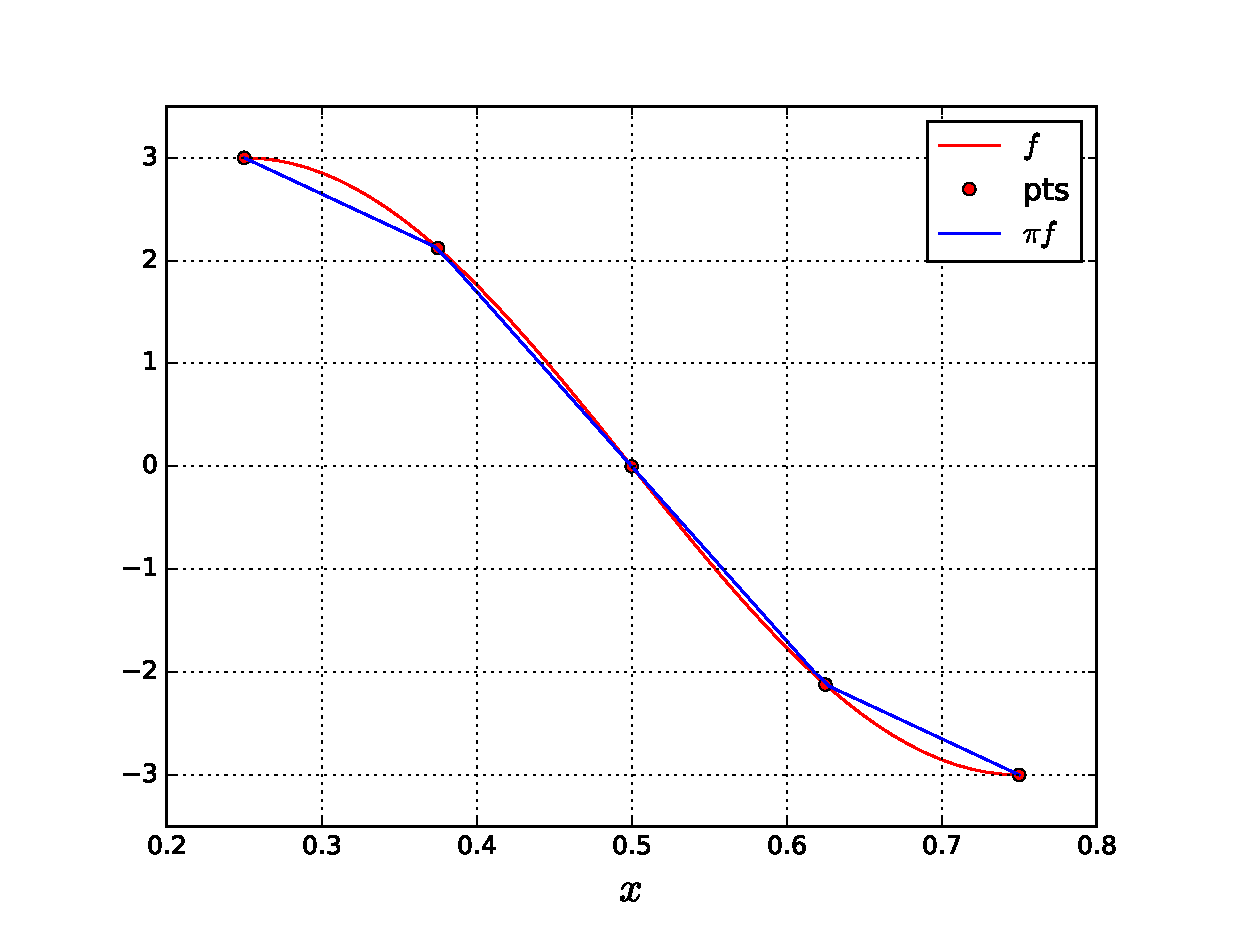
\includegraphics[width=0.8\textwidth]{./cap_mef1d/dados/ex_interp_linpartes/ex_interp_linpartes}
    \caption{Interpolação linear de $f(x)=3\sen(2\pi x)$ no espaço $V_h$ das funções lineares por partes sobre uma malha com $5$ pontos.}
    \label{fig:ex_interp_linpartes}
  \end{figure}

\ifispython
Com o \fenics, podemos computar a função interpolada $\pi f$ com o seguinte \href{https://github.com/phkonzen/notas/blob/master/src/MetodoElementosFinitos/cap_mef1d/dados/ex_interp_linpartes/ex_interp_linpartes.py}{código}:
\verbatiminput{./cap_mef1d/dados/ex_interp_linpartes/ex_interp_linpartes.py}
\fi
\end{ex}

O seguinte resultado fornece uma estimativa do erro de interpolação em relação ao tamanho $h_i$ de cada elemento da malha.

\begin{prop}\label{prop:interp_linpartes}
  O interpolador $\pi f$ satisfaz as estimativas
  \begin{align}
    \|f-\pi f\|_{L^2(I)}^2 &\leq C\sum_{i=1}^n h_i^4\|f''\|_{L^2(I)}^2,\\
    \|(f-\pi f)'\|_{L^2(I)}^2 &\leq C\sum_{i=1}^n h_i^2\|f''\|_{L^2(I)}^2.\\
  \end{align}
\end{prop}
\begin{dem}
  Ambas desigualdades seguem da desigualdade triangular e da Proposição~\ref{prop:interp_lin}. Por exemplo, para a primeira desigualdade, temos
  \begin{align}
    \|f - \pi f\|_{L^2(I)}^2 &\leq \sum_{i=1}^n \|f - \pi f\|_{L^2(I_i)}^2\\
    &\leq \sum_{i=1}^n Ch_i^4 \|f''\|_{L^2(I_i)}^2.
  \end{align}
\end{dem}

\subsection{Projeção $L^2$}

Dada uma função $f\in L^2(I)$, definimos o \emph{operador de projeção $L^2$}\index{operador de!projeção $L^2$} $P_h:L^2(I)\to V_h$ por
\begin{equation}\label{eq:proj_def}
  \int_I (f-P_hf)v\,dx=0,\quad\forall v\in V_h.
\end{equation}

Como $V_h$ é um espaço de dimensão finita, a condição \eqref{eq:proj_def} é equivalente a
\begin{equation}\label{eq:proj_def}
  \int_I (f-P_hf)\varphi_i\,dx=0,\quad i=0, 1, \cdots, n,
\end{equation}
onde $\varphi_i$ é a $i$-ésima função base de $V_h$. Além disso, como $P_hf\in V_h$, temos
\begin{equation}
  P_hf = \sum_{j=0}^n\xi_j\varphi_j,
\end{equation}
onde $\xi_j$, $j=0, 1, \dotsc, n$, são $n+1$ incógnitas a determinar. Logo,
\begin{align}
  \int_I (f-P_hf)\varphi_i\,dx=0 &\Leftrightarrow \int_I f\varphi_i\,dx = \int_I P_hf\varphi_i\,dx\\
  &\Leftrightarrow \int_I f\varphi_i\,dx = \int_I \left(\sum_{j=0}^n \xi_j\varphi_j\right)\varphi_i\,dx\\
  &\Leftrightarrow \sum_{j=0}^n \xi_j\int_I\varphi_j\varphi_i\,dx = \int_I f\varphi_i\,dx,\label{eq:proj_siseq}
\end{align}
para $i=0, 1, \dotsc, n$.

Observemos, agora, que \eqref{eq:proj_siseq} consiste em um sistema de $n+1$ equações lineares para as $n+1$ incógnitas $\xi_j$, $j=0, 1, \dotsc, n$. Este, por sua vez, pode ser escrito na seguinte forma matricial
\begin{equation}\label{eq:proj_sis}
  M\xi = b,
\end{equation}
onde $M = [m_{i,j}]_{i,j=0}^{n+1}$ é chamada de matriz de massa
\begin{equation}
  m_{i,j} = \int_I\varphi_j\varphi_i\,dx
\end{equation}
e $b = (b_0, b_1, \dotsc, b_n)$ é chamado de vetor de carregamento
\begin{equation}
  b_i = \int_I f\varphi_i\,dx.
\end{equation}

Ou seja, a projeção $L^2$ de $f$ no espaço $V_h$ é
\begin{equation}
  P_hf = \sum_{j=0}^n\xi_j\varphi_j,
\end{equation}
onde $\xi = (\xi_0, \xi_1, \dotsc, \xi_n)$ é solução do sistema \eqref{eq:proj_sis}.

\begin{ex}\label{ex:proj}
  A Figura~\ref{fig:ex_proj} ilustra a projeção $L^2$ da função $f(x)=3\sen(2\pi x)$ no espaço $V_h$ das funções lineares por partes em uma malha uniforme do intervalo $I=[1/4, 3/4]$ com $n=4$ subintervalos ($5$ pontos). 

  \begin{figure}[h!]
    \centering
    \includegraphics[width=0.8\textwidth]{./cap_mef1d/dados/ex_proj/ex_proj}
    \caption{Projeção $L^2$ de $f(x)=3\sen(2\pi x)$ no espaço $V_h$ das funções lineares por partes sobre uma malha com $5$ pontos.}
    \label{fig:ex_proj}
  \end{figure}

\ifispython
Com o \fenics, podemos computar $P_h f$ com o seguinte \href{https://github.com/phkonzen/notas/blob/master/src/MetodoElementosFinitos/cap_mef1d/dados/ex_proj/ex_proj.py}{código}:
\verbatiminput{./cap_mef1d/dados/ex_proj/ex_proj.py}
\fi
\end{ex}

O próximo teorema mostra que $P_h f$ é a função que melhor aproxima $f$ dentre todas as funções do espaço $V_h$.

\begin{teo}(\normalfont{A melhor aproximação.})\label{teo:melho_aprox}
  A projeção $L^2$ satisfaz
  \begin{equation}
    \|f-P_hf\|_{L^2(I)} \leq \|f - v\|_{L^2(I)},\quad\forall v\in V_h.
  \end{equation}
\end{teo}
\begin{dem}
  Dado $v\in V_h$, temos
  \begin{align}
    \|f-P_hf\|_{L^2(I)}^2 &= \int_I |f-P_hf|^2\,dx\\
    &= \int_I (f-P_hf)(f-v+v-P_hf)\,dx\\
    &= \int_I(f-P_hf)(f-v)\,dx + \int_I(f-P_hf)(v-P_hf)\,dx\\
    &= \int_I (f-P_hf)(f-v)\,dx\\
    &\leq \int_I \|f-P_hf\|_{L^2(I)}\|f-v\|_{L^2(I)},
  \end{align}
donde segue o resultado.
\end{dem}

O próximo teorema fornece uma estimativa {\it a-priori} do erro $\|f-P_h f\|_{L^2(I)}$ em relação ao tamanho da malha.

\begin{teo}
  A projeção $L^2$ satisfaz
  \begin{equation}
    \|f-P_hf\|_{L^2(I)} \leq C\sum_{i=1}^n h_i^4\|f''\|_{L^2(I_i)}^2.
  \end{equation}
\end{teo}
\begin{dem}
  Tomando a interpolação $\pi f \in V_h$, temos do Teorema da melhor aproximação (Teorema \ref{teo:melhor_aprox}) e da estimativa do erro de interpolação (Proposição \ref{prop:interp_linpartes}) que
  \begin{align}
    \|f - P_hf\|_{L^2(I)}^2 &\leq \|f-\pi f\|_{L^2(I)}^2\\
    &\leq C\sum_{i=1}^n h_i^4\|f''\|_{L^2(I_i)}^2.
  \end{align}
\end{dem}

\emconstrucao

\subsection{Exercícios}

\begin{exer}
  Faça um código para verificar a segunda estimativa da Proposição~\ref{prop:interp_lin} no caso da interpolação da função $f(x) = 3\sen(2\pi x)$ no espaço $P_1$ das funções lineares.
\end{exer}


\begin{exer}
  Faça um código para verificar as estimativas da Proposição~\ref{prop:interp_linpartes} no caso da interpolação da função $f(x) = 3\sen(2\pi x)$ no espaço $V_h$ das funções lineares por partes.
\end{exer}

\emconstrucao
%Este trabalho está licenciado sob a Licença Atribuição-CompartilhaIgual 4.0 Internacional Creative Commons. Para visualizar uma cópia desta licença, visite http://creativecommons.org/licenses/by-sa/4.0/deed.pt_BR ou mande uma carta para Creative Commons, PO Box 1866, Mountain View, CA 94042, USA.

\chapter{Problemas Bidimensionais}\label{cap_mef2d}
\thispagestyle{fancy}

\section{Malha e Espaço}\label{cap_mef2d_sec_malha}
\badgeRevisar

\subsection{Malha}
\badgeRevisar

Seja $\Omega\subset \mathbb{R}^2$ um domínio limitado com fronteira $\p\Omega$ suave e poligonal. Uma \hlemph{malha (ou triangularização) $\mathcal{K}$ de $\Omega$ é um conjunto de $\{K\}$ células (ou elementos) $K$, em que $\Omega = \cup_{K\in\mathcal{K}}K$ e tal que a interseção de duas células é ou um lado, um canto ou vazio}.

Classicamente as células $K$ são escolhidas como triângulos. \hl{O comprimento do maior lado da célula $K$ define o chamado \emph{tamanho local da malha} $h_K$}. O \hl{\emph{tamanho global da malha} é definida por $h = \max_{K\in\mathcal{K}} h_K$}.

Uma \hlemph{malha} é dita \hl{\emph{regular} quando existe uma constante $c_0 > 0$ tal que $c_K > c_0$ para todo $K\in\mathcal{K}$, sendo $c_K := d_K/h_K$ e $d_K$ o diâmetro do circulo inscrito em $K$}. Esta condição significa que os triângulos $K$ da malha não podem ter ângulos muito grandes nem muito pequenos. \hl{Ao longo do texto}, a menos que especificado o contrário, \hl{assumiremos trabalhar com \emph{malhas regulares}}.

\begin{ex}\label{cap_mef2d_sec_malha:ex:malha}
 O seguinte código, gera uma malha uniforme no domínio $\Omega = [0, 1]^2$.

 \begin{figure}[H]
  \centering
  \includegraphics[width=0.7\textwidth]{./cap_mef2d/dados/ex_malha/fig}
  \caption{Esboço de uma malha triangular no domínio $D = [0, 1]^2$.}
  \label{cap_mef2d_sec_malha:fig:ex_malha}
\end{figure}

 
\begin{lstlisting}[caption=ex\_malha.py]
from mpi4py import MPI
from dolfinx import mesh

# malha triangular
domain = mesh.create_unit_square(MPI.COMM_WORLD, 
                                  nx = 5, ny = 5)

# gráfico da malha
import pyvista
# pyvista.set_jupyter_backend('static')
print(pyvista.global_theme.jupyter_backend)

from dolfinx import plot
pyvista.start_xvfb()
tdim = domain.topology.dim
topology, cell_types, geometry = plot.vtk_mesh(domain, tdim)
grid = pyvista.UnstructuredGrid(topology, cell_types, geometry)

plotter = pyvista.Plotter()
plotter.add_mesh(grid, show_edges=True)
plotter.view_xy()
pyvista.OFF_SCREEN=True
if not pyvista.OFF_SCREEN:
    plotter.show()
else:
    figure = plotter.screenshot("malha.png")  
\end{lstlisting}
\end{ex}


\subsection{Espaço de Polinômios Lineares}
\badgeRevisar

Seja $K$ um triângulo e seja \hl{$P_1(K)$ o \emph{espaço dos polinômios lineares} em $K$}, i.e.
\begin{equation}\hleq
  \begin{aligned}
    &P_1(K) = \{v;~v=c_0+c_1x_0+c_2x_1,\\
    &\qquad\qquad\qquad(x_0,x_1)\in K,~c_0,c_1,c_2\in\mathbb{R}\}.
  \end{aligned}
\end{equation}

Observamos que \hl{toda função $v\in P_1(K)$ é unicamente determinada por seus valores nodais} 
\begin{equation}\label{cap_mef2d_sec_malha:eq:sis_aux}
  \alpha_i = v(N_i), i=0, 1, 2,
\end{equation} 
onde $N_i = (x_0^{(i)}, x_1^{(i)})$ é o $i$-ésimo nodo (vértice) do triângulo $K$. Isto segue do fato de que o sistema \eqref{cap_mef2d_sec_malha:eq:sis_aux} tem forma matricial
\begin{equation}
  \begin{bmatrix}
    1 & x_0^{(0)} & x_1^{(0)}\\
    1 & x_0^{(1)} & x_1^{(1)}\\
    1 & x_0^{(2)} & x_1^{(2)}
  \end{bmatrix}
  \begin{bmatrix}
    c_0\\
    c_1\\
    c_2
  \end{bmatrix} = 
  \begin{bmatrix}
    \alpha_0\\
    \alpha_1\\
    \alpha_2
  \end{bmatrix}
\end{equation}
Ainda, o valor absoluto do determinante da matriz de coeficientes é $2|K|$, onde $|K|$ denota a área de $K$, a qual é não nula.

Afim de usarmos os valores nodais como graus de liberdade (incógnitas), nós introduzimos a seguinte base nodal $\{\lambda_0, \lambda_1, \lambda_2\}$ com
\begin{equation}
  \lambda_j(N_i) = \left\{
    \begin{array}{ll}
      1 &, i=j,\\
      0 &, i\neq j
    \end{array}
\right.,~i,j=0,1,2.
\end{equation}
Com esta base, toda função $v\in P_1(K)$ pode ser escrita como
\begin{equation}
  v = \alpha_0\lambda_0 + \alpha_1\lambda_1 + \alpha_2\lambda_2,
\end{equation}
onde $\alpha_i = v(N_i)$.

\subsection{Espaço contínuo dos polinômios lineares por partes}
\badgeRevisar

O \hl{\emph{espaço contínuo dos polinômios lineares por partes} na malha $\mathcal{K}$ é definido por}
\begin{equation}\hleq
  V_h = \{v;~v\in C^0(\Omega),~v|_K\in P_1(K),~\forall K\in\mathcal{K}\}.
\end{equation}

Observamos que \hl{toda função $v\in V_h$ é unicamente determinada por seus valores nodais} $\{v(N_j)\}_{j=0}^{n_p-1}$, onde $n_p$ é número de nodos da malha $\mathcal{K}$. 

De fato, os valores nodais determinam uma única função em $P_1(K)$ para cada $K\in\mathcal{K}$ e, portanto, uma função em $V_h$ é unicamente determinada por seus valores nos nodos. Agora, consideremos dois triângulos $K_1$ e $K_2$ compartilhando um lado $E = K_1\cap K_2$. Sejam $v_1$ e $v_2$ os dois únicos polinômios em $v_1\in P_1(K_1)$ e $v_2\in P_1(K_2)$, respectivamente determinados pelos valores nodais em $K_1$ e $K_2$. Como $v_1$ e $v_2$ também são polinômios lineares em $E$ e seus valores coincidem nos nodos de $E$, temos $v_1 = v_2$ em $E$. Portanto, concluímos que toda função $v\in V_h$ é unicamente determinada por seus valores nodais.

Afim de termos os valores nodais como graus de liberdade (incógnitas), definimos a \hlemph{base nodal} $\{\varphi_j\}_{j=1}^{n_p}\subset V_h$ tal que
\begin{equation}\hleq
  \varphi_j(N_i) = \left\{
    \begin{array}{ll}
      1 &, i=j\\
      0 &, i\neq j
    \end{array}
\right.,~i,j=0, 1, \dotsc, n_p-1.
\end{equation}
Notamos que \hl{cada função base $\varphi_j$ é contínua, polinômio linear por partes e com suporte somente em um pequeno conjunto de triângulos que compartilham o nodo $N_j$}. Além disso, \hl{toda a função $v\in V_h$ pode, então, ser escrita como}
\begin{equation}\hleq
  v = \sum_{i=0}^{n_p-1}\alpha_i\varphi_i,
\end{equation}
onde $\alpha_i = v(N_i)$, $i=0, 1, \ldots, n_p$, são os valores nodais de $v$.

\begin{ex}\label{cap_mef2d_sec_malha:ex:espaço}
No seguinte código, alocamos um espaço de elementos finitos $V_h$ sobre uma malha regular no domínio $\Omega=[0,1]^2$. Ainda, uma função $u_h\in V_h$ é alocada com valores nodais
\begin{equation}
  u(\pmb{x}) = \sen(\pi x_0)\sen(\pi x_1).
\end{equation}

\begin{figure}
  \centering
  \includegraphics[width=0.8\textwidth]{./cap_mef2d/dados/ex_espaco/fig}
  \caption{Esboço de uma função no espaço $V_h$ com valores nodais $u(\pmb{x}) = \sen(\pi x_0)\sen(\pi x_1)$.}
\end{figure}

\begin{lstlisting}
from mpi4py import MPI
from dolfinx import mesh

# malha
domain = mesh.create_unit_square(MPI.COMM_WORLD, 5, 5)

from dolfinx import fem

# espaço de elementos finitos
V = fem.functionspace(domain, ("P",1))

# função do espaço V
uh = fem.Function(V)

# valor nodais
from numpy import sin, pi
for i,x in enumerate(domain.geometry.x):
  uh.x.array[i] = sin(pi*x[0])*sin(pi*x[1])

# gráfico
u_topology, u_cell_types, u_geometry = plot.vtk_mesh(V)
u_grid = pyvista.UnstructuredGrid(u_topology, u_cell_types, u_geometry)
u_grid.point_data["u"] = uh.x.array.real
u_grid.set_active_scalars("u")
u_plotter = pyvista.Plotter()
u_plotter.add_mesh(u_grid, show_edges=True)
u_plotter.view_xy()
if not pyvista.OFF_SCREEN:
  u_plotter.show()
else:
  figure = u_plotter.screenshot("u.png")
\end{lstlisting}
\end{ex}

\subsection{Exercícios}
\badgeConstrucao

\section{Interpolação}\label{cap_mef2d_sec_interp}
\badgeRevisar

Dada uma função contínua $f$ em um triângulo $K$ com nodos $N_i$, $i=0, 1, 2$, sua interpolação linear $\pi f \in P_1(K)$ é definida por
\begin{equation}
  \pi f = \sum_{i=0}^3 f(N_i)\varphi_i.
\end{equation}
Logo, temos $\pi f(N_i) = f(N_i)$ para todo $i=0, 1, 2$.

\begin{ex}\label{cap_mef2d_sec_interp:ex:interp2d}
  Consideramos a função
  \begin{equation}
    u(x_0, x_1) = \sen(\pi x_0)\cos(\pi x_1)
  \end{equation}
  defina no domínio $D = [0,1]^2$. O seguinte código computa a interpolação de $f$ no espaço de elementos finitos $V_h$ sobre uma malha uniforme de $16\times 16$ triângulos. Com ele, graficamos a função interpolada $u_h\in V_h$ e a função $u$. Consulte a Fig.~\ref{cap_mef2d_sec_interp:fig:interp2d}.

  \begin{figure}
    \centering
    \includegraphics[width=0.8\textwidth]{cap_mef2d/dados/ex_interp/fig}
    \caption{Gráfico de comparação função interpolada $u_h\in V_h$ (gráfico de contornos em cores) e da função original $u$ (isolinhas) referentes ao Exemplo~\ref{cap_mef2d_sec_interp:ex:interp2d}.}
    \label{cap_mef2d_sec_interp:fig:interp2d}
  \end{figure}

\begin{lstlisting}[caption=interp2d.py, label=cap_mef2d_sec_interp:cod:interp2d]
from mpi4py import MPI
from dolfinx import mesh

# malha
domain = mesh.create_unit_square(MPI.COMM_WORLD, 16, 16)

from dolfinx import fem

# espaço de elementos finitos
V = fem.functionspace(domain, ("P",1))

# função do espaço V
uh = fem.Function(V)

# interpolate
import numpy as np
def u(x, mod=np):
    return mod.sin(mod.pi*x[0])*mod.sin(mod.pi*x[1])

uh.interpolate(lambda x: u(x))

# eval fun
from dolfinx import geometry

def fun_eval(u, points,
             domain=domain):
  u_values = []
  bb_tree = geometry.bb_tree(domain, domain.topology.dim)
  cells = []
  points_on_proc = []
  # Find cells whose bounding-box collide with the the points
  cell_candidates = geometry.compute_collisions_points(bb_tree, 
                                                       points.T)
  # Choose one of the cells that contains the point
  colliding_cells = geometry.compute_colliding_cells(domain, 
                                                     cell_candidates, 
                                                     points.T)
  for i, point in enumerate(points.T):
    if len(colliding_cells.links(i)) > 0:
      points_on_proc.append(point)
      cells.append(colliding_cells.links(i)[0])

  points_on_proc = np.array(points_on_proc, dtype=np.float64)
  u_values = u.eval(points_on_proc, cells)
  return u_values

# gráfico
import numpy as np
nx = ny = 101
xx0 = np.linspace(0., 1., nx)
xx1 = np.linspace(0., 1., ny)
X0, X1 = np.meshgrid(xx0, xx1, indexing='ij')
points = np.zeros((3, nx*ny))
points[0] = X0.reshape(-1)
points[1] = X1.reshape(-1)

yh = fun_eval(uh, points)
Yh = yh.reshape((nx,ny))

import matplotlib.pyplot as plt

fig = plt.figure()
ax = fig.add_subplot()
levels=10
cb = ax.contourf(X0, X1, Yh, levels = levels)
fig.colorbar(cb)
Y = u([X0, X1])
cl = ax.contour(X0, X1, Y, levels = levels, colors='w')
ax.clabel(cl)
plt.show()
\end{lstlisting}
\end{ex}

Afim de determinarmos estimativas para o erro de interpolação, precisamos da chamada derivada total de primeira ordem
\begin{equation}
  Df = \left(\left|\frac{\p f}{\p x_0}\right|^2 + \left|\frac{\p f}{\p x_1}\right|^2\right)^{1/2},
\end{equation}
e da derivada total de segunda ordem
\begin{equation}
  D^2f = \left(\left|\frac{\p^2 f}{\p x_0^2}\right|^2 + \left|\frac{\p^2 f}{\p x_0\p x_1}\right|^2 + \left|\frac{\p^2 f}{\p x_1^2}\right|^2\right)^{1/2}.
\end{equation}

\begin{prop}\normalfont{(\hl{Erro da interpolação no espaço linear}.)}\label{prop:interpl}
  A interpolação $\pi f$ satisfaz as seguintes estimativas
  \begin{align}
    \|f - \pi f\|_{L^2(K)} &\leq Ch_K^2\|D^2f\|_{L^2(K)},\label{eq:interpl_0}\\
    \|D(f - \pi f)\|_{L^2(K)} &\leq Ch_K\|D^2 f\|_{L^2(K)}.\label{eq:interpl_1}
  \end{align}
\end{prop}
\begin{dem}
  Veja \cite[Capítulo 4]{Brenner2008a}.
\end{dem}

\begin{obs}
  A constante $C$ dependo do inverso de $\sen(\theta_K)$ onde $\theta_K$ é o menor angulo de $K$. Desta forma, para um triângulo com $\theta_K$ muito pequeno, as estimativas \eqref{eq:interpl_0} e \eqref{eq:interpl_1} perdem sentido. Este fato indica a necessidade de se trabalhar com malhas regulares.
\end{obs}

A interpolação no espaço $V_h$ de uma dada função $f$ no domínio $\Omega$ é denotada também por $\pi f\in V_h$ e definida por
\begin{equation}
  \pi f = \sum_{i=0}^{n_p-1} f(N_i)\varphi_i.
\end{equation}

\begin{prop}\normalfont{(\hl{Erro da interpolação no espaço contínuo linear por partes}.)}\label{prop:interpc}
  O interpolador $\pi f\in V_h$ satisfaz as seguintes estimativas
  \begin{align}
    &\|f - \pi f\|_{L^2(\Omega)}^2 \leq C\sum_{K\in\mathcal{K}} h_K^4\|D^2 f\|_{L^2(K)}^2,\label{eq:interpc_0}\\
    &\|D(f - \pi f)\|_{L^2(\Omega)}^2 \leq C\sum_{K\in\mathcal{K}} h_K^2\|D^2 f\|_{L^2(K)}^2,\label{eq:interpc_1}.
  \end{align}
\end{prop}
\begin{dem}
  Demonstração análoga a Proposição \ref{prop:interp_linpartes}.
\end{dem}

\begin{obs}\normalfont{(\hl{Taxa de convergência}.)}
  A taxa de convergência (ou ordem de truncamento) do erro de interpolação é definida como a potência do $h$ na estimativa \eqref{eq:interpc_0}. Esta taxa pode ser computacionalmente estimada. De fato, o erro de interpolação para uma dada malha $i$ tem a forma $\varepsilon_i \approx Ch_i^{r}$. Conhecendo $\varepsilon_{i-1} \approx Ch_{i-1}^{r}$ para uma outra malha $i-1$, podemos resolver para $r$, obtendo a estimativa
  \begin{equation}\label{cap_mef2d_sec_interp:eq:conv_est}
    r \approx \frac{\ln{\varepsilon_i/\varepsilon_{i-1}}}{\ln{h_i/h_{i-1}}}.
  \end{equation}
\end{obs}

\begin{ex}\label{cap_mef2d_sec_interp:ex:interp_err}
  Consideramos a interpolação feita no Exemplo~\ref{cap_mef2d_sec_interp:ex:interp2d}. Aqui, computamos o erro de interpolação na norma $L^2$, i.e.
  \begin{equation}
    \varepsilon = \|u_h - u\|_{L^2(\Omega)}
  \end{equation}
  para diferentes refinamentos de malha. 

  \begin{figure}[H]
    \centering
    \includegraphics[width=0.8\textwidth]{cap_mef2d/dados/ex_interp_err/fig}
    \caption{Tamanho da malha $h$ \textit{versus} erro de interpolação na norma $L^2$ referente ao Exemplo~\ref{cap_mef2d_sec_interp:ex:interp_err}.}
  \end{figure}

  Na Tabela~\ref{cap_mef2d_sec_interp:tab:interp_err}, temos o número de células e seu tamanho $h$, o erro de interpolação $\varepsilon$ e a estimativa da taxa de convergência dada por \eqref{cap_mef2d_sec_interp:eq:conv_est}.

  \begin{table}[H]
    \centering
    \caption{Erro de interpolação referente ao Exemplo~\ref{cap_mef2d_sec_interp:ex:interp_err}.}
    \begin{tabular}{cr|rr}\toprule
      \#células & $h$ & $\epsilon$ & $r$ \\\midrule
      $4\times 4$ & $3.5\times 10^{-1}$ & $6.0\times 10^{-2}$ & -x-\\
      $8\times 8$ & $1.8\times 10^{-1}$ & $1.6\times 10^{-2}$ & 1.91\\
      $16\times 16$ & $8.8\times 10^{-2}$ & $3.9\times 10^{-3}$ & 2.04 \\
      $32\times 32$ & $4.4\times 10^{-2}$ & $9.8\times 10^{-4}$ & 1.99\\
      $64\times 64$ & $2.2\times 10^{-2}$ & $2.4e\times 10^{-4}$ & 2.03\\\bottomrule
    \end{tabular}
    \label{cap_mef2d_sec_interp:tab:interp_err}
  \end{table}
\end{ex}

\subsection{Exercícios}
\badgeConstrucao

\section{Projeção}\label{cap_mef2d_sec_proj}
\badgeRevisar

\hl{A \emph{projeção} $L^2$ no espaço $V_h$ de uma dada uma função $u\in L^2(\Omega)$ \emph{é denotada por} $P_hu\in V_h$ \emph{e definida por}}
\begin{equation}\hleq
  \int_\Omega (u-P_hu)v\,dx = 0,~\forall v\in V_h.
\end{equation}

Analogamente a projeção em uma dimensão (consulte Subseção \ref{subsec:projecao_1d}), a projeção é dada por
\begin{equation}\hleq
  P_h u = \sum_{j=0}^{n_p-1} \xi_j\varphi_j,
\end{equation}
com $\pmb{\xi} = (\xi_j)_{j=0}^{n_p-1}$ satisfazendo o sistema linear
\begin{equation}\hleq
  M\pmb{\xi} = \pmb{b},
\end{equation}
onde $M = [m_{i,j}]_{i,j=0}^{n_p-1}$ é a \emph{matriz de massa} com
\begin{equation}\hleq
  m_{i,j} = \int_{\Omega} \varphi_i\varphi_j\,dx
\end{equation}
e $\pmb{b} = (b_1,~b_2,~\dotsc,~b_{n_p-1})$ é o \emph{vetor de carga} com
\begin{equation}\hleq
  b_i = \int_\Omega u\varphi_i\,dx.
\end{equation}

Também, vale o resultado análogo da \hlemph{melhor aproximação} (consulte Teorema~\ref{teo:melhor_aprox}), i.e.
\begin{equation}\hleq
  \|u-P_hu\|_{L^2(\Omega)} \leq \|u - v\|_{L^2(\Omega)},\quad\forall v\in V_h.
\end{equation}
E, portanto, também temos a estimativa análoga para o \hlemph{erro de projeção} (condulte Teorema~\ref{teo:erro_proj_1d})
\begin{equation}\hleq
  \|u-P_hu\|_{L^2(\Omega)}^2 \leq C\sum_{K\in\mathcal{K}} h_K^4\|D^2 u\|_{L^2(K)}^2.
\end{equation}
Tomando o tamanho global da malha, temos
\begin{equation}\label{eq:erro_projec_2d}\hleq
  \|f-P_hf\|_{L^2(\Omega)} \leq Ch^2\|D^2 f\|_{L^2(K)}.
\end{equation}

\begin{ex}\label{cap_mef2d_sec_proj:ex:proj}
Consideramos a função $u(x_0,x_1) = \sen(\pi x_0)\cos(\pi x_1)$ definida no domínio $D = [0, 1]\times [0, 1]$. código computa a projeção de $u$ no espaço $V_h$ sobre uma malha triangular uniforme.
\begin{lstlisting}
from mpi4py import MPI
from dolfinx import mesh

# malha
domain = mesh.create_unit_square(MPI.COMM_WORLD, 16, 16)

from dolfinx import fem

# espaço de elementos finitos
Vh = fem.functionspace(domain, ("P",1))

# função do espaço V
uh = fem.Function(Vh)

# projeção
import ufl
from dolfinx.fem.petsc import LinearProblem
def uex(x, mod=ufl):
    return mod.sin(mod.pi*x[0])*mod.sin(mod.pi*x[1])

x = ufl.SpatialCoordinate(domain)
u = ufl.TrialFunction(Vh)
v = ufl.TestFunction(Vh)
a = ufl.dot(u,v)*ufl.dx
L = uex(x)*v*ufl.dx
problem = LinearProblem(a, L, bcs=[])
Phu = problem.solve()

# saída (paraview)
from dolfinx import io
from pathlib import Path
results_folder = Path("results")
results_folder.mkdir(exist_ok=True, parents=True)
filename = results_folder / "phu"
Phu.name = "Phu"
with io.VTXWriter(domain.comm, filename.with_suffix(".bp"), [Phu]) as vtx:
    vtx.write(0.0)
with io.XDMFFile(domain.comm, filename.with_suffix(".xdmf"), "w") as xdmf:
    xdmf.write_mesh(domain)
    xdmf.write_function(Phu, 0.0)
\end{lstlisting}
\end{ex}

\subsection{Exercícios}
\badgeRevisar

\begin{exer}
  Verifique computacionalmente a estimativa \eqref{eq:erro_projec_2d} no caso da função $f(x_0,x_1) = \sen(\pi x_0)\cos(\pi x_1)$ projetada sobre uma malha triangular uniforme sobre o domínio $D = [0, 1]\times [0, 1]$.
\end{exer}

\section{Problema modelo}\label{cap_mef2d_sec_probmodelo}
\badgeRevisar

Nesta seção, apresentaremos a aplicação do método de elementos finitos para a equação de Poisson\footnote{Siméon Denis Poisson, 1781 - 1840, matemático francês. Fonte: \href{https://en.wikipedia.org/wiki/Sim\%C3\%A9on_Denis_Poisson}{Wikipedia}.} com condições de Dirichlet\footnote{Johann Peter Gustav Lejeune Dirichlet, 1805 - 1859, matemático alemão. Fonte: \href{https://en.wikipedia.org/wiki/Peter_Gustav_Lejeune_Dirichlet}{Wikipedia}.}, i.e.: encontrar $u$ tal que
\begin{align}
  -\Delta u &= f,~x\in\Omega,\label{eq:mef2d_pm_eq}\\
  u &= 0,~x\in\p\Omega,\label{eq:mef2d_pm_bc}
\end{align}
onde $\Delta = \p^2/\p x_0^2 + \p^2/\p x_1^2$ é o operador de Laplace\footnote{Pierre-Simon, marquis de Laplace, 1749 - 1827, matemático francês. Fonte: \href{https://en.wikipedia.org/wiki/Pierre-Simon_Laplace}{Wikipedia}.} e $f$ é uma função dada.

\subsection{Formulação variacional}
\badgeRevisar

A aplicação do método de elementos finitos é construída sobre a formulação fraca do problema \eqref{eq:mef2d_pm_eq}-\eqref{eq:mef2d_pm_bc}. Para obtermos esta, multiplicamos \eqref{eq:mef2d_pm_eq} por uma função teste $v$ em um espaço adequado $V_0$ e integramos no domínio $\Omega$, i.e.
\begin{equation}
  - \int_\Omega \Delta uv\,dx = \int_\Omega fv\,dx.
\end{equation}
Então, usando a fórmula de Green\footnote{George Green, 1793 - 1841, matemático britânico. Fonte: \href{https://en.wikipedia.org/wiki/George_Green_(mathematician)}{Wikipedia}.}, obtemos
\begin{equation}
  \int_\Omega \nabla u\cdot\nabla v\,dx - \int_{\p\Omega} n\cdot\nabla uv\,ds.
\end{equation}
Então, observando critérios de regularidade e a condição de contorno \eqref{eq:mef2d_pm_bc}, escolhemos
\begin{equation}
  V_0 := \{v\in H^1(\Omega):~v|_{\p\Omega}=0\}.
\end{equation}
Lembramos que $H^1(\Omega) = \{v:~\|v\|_{L^2(\Omega)}+\|\nabla v\|_{L^2(\Omega)}<\infty\}$.

Com isso, temos o seguinte problema fraco associado a \eqref{eq:mef2d_pm_eq}-\eqref{eq:mef2d_pm_bc}: encontrar $u\in V_0$ tal que
\begin{equation}\label{eq:mef2d_probfraco}
  a(u,v) = L(v),~\forall v\in V_0,
\end{equation}
onde $a(u, v)$ é chamada de forma bilinear e definida por
\begin{equation}
  a(u,v) := \int_\Omega \nabla u\cdot\nabla v\,dx
\end{equation}
e $L(v)$ é chamada de forma linear e definida por
\begin{equation}
  L(v) := \int_\Omega fv\,dx.
\end{equation}

\subsection{Formulação de elementos finitos}
\badgeRevisar

A formulação de elementos finitos é obtida da formulação fraca \eqref{eq:mef2d_probfraco} pela aproximação do espaço teste $V_0$ por uma espaço de dimensão finita. Tomando uma triangulação $\mathcal{K}\subset\Omega$ e considerando o espaço contínuo dos polinômios lineares por partes
\begin{equation}
  V_h := \{v:~v\in C^0(\Omega), v|_K\in P_1(K)~\forall K\in\mathcal{K}\},
\end{equation}
assumimos também o subconjunto $V_{h,0}:= \{v\in V_h:~v|_{\p\Omega}=0\}$.

Com isso, temos o seguinte problema de elementos finitos associado \eqref{eq:mef2d_probfraco}: encontrar $u_h\in V_{h,0}$ tal que
\begin{equation}\label{eq:mef2d_probfem}
  a(u_h,v_h) = L(v_h),~\forall v_h\in V_{h,0}.
\end{equation}

Observemos que \eqref{eq:mef2d_probfem} é equivalente ao problema de encontrar $u_h\in V_{h,0}$ tal que
\begin{equation}\label{eq:mef2d_proba1}
  a(u_h,\varphi_i) = L(\varphi_i),
\end{equation}
com $i=0, 1, \cdots, n_p-1$, onde $\{\varphi_i\}_{i=0}^{n_i-1}$ é a base nodal de $V_{h,0}$ e $n_i$ é o número de funções bases (igual ao número de nodos internos da triangulação $\mathcal{K}$). Ainda, como
\begin{equation}
  u_h = \sum_{j=0}^{n_i-1} \xi_j\varphi_j,
\end{equation}
temos 
\begin{align}
  a(u_h, \varphi_i) &= a\left(\sum_{j=0}^{n_i-1}\xi_j\varphi_j,\varphi_i\right) \\
  &= \sum_{j=0}^{n_i-1}\xi_ja(\varphi_j,\varphi_i).
\end{align}

Com isso, o problema de elementos finitos é equivalente a resolver o seguinte sistema linear
\begin{equation}
  \sum_{j=0}^{n_i-1}\xi_ja(\varphi_j,\varphi_i) = L(\varphi_i),~i=0, 1, \cdots, n_i-1,
\end{equation}
para as incógnitas $\xi_j$, $j=0, 1, \cdots, n_i-1$. Ou, equivalentemente, temos sua forma matricial
\begin{equation}
  A\pmb{\xi} = \pmb{b},
\end{equation}
onde $A = [a_{i,j}]_{i,j=0}^{n_i-1}$ é chamada de \pmb{matriz de rigidez}\index{matriz de rigidez} com
\begin{equation}
  a_{i,j} = a(\varphi_j, \varphi_i)
\end{equation}
e $\pmb{b} = (b_0, b_1, \cdots, b_{n_i-1})$ é o vetor de carga com
\begin{equation}
  b_i = L(\varphi_i).
\end{equation}

\begin{ex}\label{ex:mef2d_pm}
  Consideremos o seguinte problema de Poisson
  \begin{align}
    -\Delta u &= 100x_0(1-x_0)x_1(1-x_1),~x\in\Omega:=(0, 1)\times (0, 1),\\
    u &= 0,~x\in\p\Omega.
  \end{align}
  Na Figura \ref{fig:mef2d_pm} temos um esboço da aproximação de elementos finitos obtida em uma malha uniforme com $20\times 20$ nodos. As isolinhas correspondem aos ponto tais que $u=3\times 10^{-1}, 2\times 10^{-1}$, $10^{-1}$, $5\times 10^{-2}$.

  \begin{figure}[h!]
    \centering
    \includegraphics[width=0.7\textwidth]{./cap_mef2d/dados/ex_mef2d_pm/fig_mef2d_pm}
    \caption{Esboço da solução de elementos finitos do problema discutido no Exemplo \ref{ex:mef2d_pm}.}
    \label{fig:mef2d_pm}
  \end{figure}

\ifispython
Com o \fenics, podemos computar a solução deste problema com o seguinte \href{https://github.com/phkonzen/notas/blob/master/src/MetodoElementosFinitos/cap_mef2d/dados/ex_mef2d_pm/ex_mef2d_pm.py}{código}:
\verbatiminput{./cap_mef2d/dados/ex_mef2d_pm/ex_mef2d_pm.py}
\fi
\end{ex}

\subsection{Exercícios}
\badgeRevisar

\begin{exer}
  Compute uma aproximação de elementos finitos para o seguinte problema
\begin{align}
  -\Delta u &= 10,~x\in (0, 1)\times (0, 1)\\
  u(x,0) &= 0,~0\leq x \leq 1,\\
  u(1,y) &= 0,~0\leq y < 1,\\
  u(x,1) &= 1,~0\leq x \leq 1,\\
  u(0,y) &= 1,~0<x\leq 1.
\end{align}
\end{exer}

\section{Fundamentos da análise de elementos finitos}\label{cap_mef2d_sec_funanlef}
\badgeRevisar

\subsection{Existência e unicidade}
\badgeRevisar

\begin{teo}\normalfont{(Matriz positiva definida)}\label{teo:matriz_definida_positiva}
  A matriz de rigidez é positiva definida.
\end{teo}
\begin{dem}
  A matriz de rigidez $A = [a(\varphi_j,\varphi_i)]_{ij=0}^{n_i-1}$ é obviamente simétrica. Além disso, para todo $\pmb{\xi}\in\mathbb{R}^{n_i}$, $\pmb{\xi}\neq 0$, temos
  \begin{align}
    \pmb{\xi}^TA\pmb{\xi} &= \sum_{i,j=0}^{n_i-1} \xi_ja(\varphi_j,\varphi_i)\xi_i\\
    &= \sum_{i,j=0}^{n_i-1}\xi_j\int_\Omega \nabla \varphi_j\cdot\nabla\varphi_i\,dx\,\xi_i\\
    &= \int_\Omega \nabla \left(\sum_{j=0}^{n_i-1}\xi_j\varphi_j\right)\cdot\nabla \left(\sum_{i=0}^{n_i-1}\xi_i\varphi_i\right)\,dx\\
    &= \left\|\nabla \left(\sum_{j=0}^{n_i-1}\xi_j\varphi_j\right) \right\|_{L^2(\Omega)}^2.
  \end{align}
  Portanto, $\pmb{\xi}^TA\pmb{\xi} \geq 0$ e é nulo se, e somente se, $v = \sum_{j=0}^{n_i-1}\xi_j\varphi_j$ for constante. Como $v\in V_{h,0}$, temos que $v$ constante implica $v\equiv 0$, mas então $\pmb{\xi}=0$, o que é uma contradição. Logo, $\pmb{\xi}^TA\pmb{\xi} > 0$ para todo $\pmb{\xi}\in\mathbb{R}^{n_i}$, $\pmb{\xi}\neq 0$.
\end{dem}

\begin{teo}\normalfont{(Existência e unicidade)}
  O problema de elementos finitos \eqref{eq:mef2d_probfem} tem solução única.
\end{teo}
\begin{dem}
  O problema de elementos finitos \eqref{eq:mef2d_probfem} se resume a resolver o sistema linear $A\pmb{\xi} = \pmb{b}$. Do Teorema \ref{teo:matriz_definida_positiva}, temos que $A$ é uma matriz definida positiva e, portanto, invertível. Daí segue, imediatamente, que o problema \eqref{eq:mef2d_probfem} tem solução única.
\end{dem}

\subsection{Estimativa {\it a priori} do erro}
\badgeRevisar

\begin{teo}\normalfont{(Ortogonalidade de Galerkin)}\label{teo:mef2d_orto_Galergin}
  A solução $u_h$ do problema de elementos finitos \eqref{eq:mef2d_probfem} satisfaz
  \begin{equation}
    a(u-u_h,v_h) = 0,~\forall v_h\in V_{h,0},
  \end{equation}
onde $u$ é a solução do problema fraco \eqref{eq:mef2d_probfraco}.
\end{teo}
\begin{dem}
  Segue, imediatamente, do fato de que $V_{h,0}\subset V_0$ e, portanto,
  \begin{equation}
    a(u,v_h) = L(v_h),~\forall v_h\in V_{h,0},
  \end{equation}
bem como
  \begin{equation}
    a(u_h,v_h) = L(v_h),~\forall v_h\in V_{h,0}.
  \end{equation}
\end{dem}

\begin{defn}\normalfont{(Norma da energia.)}
  Definimos a norma da energia por
  \begin{equation}
    \||v|\| := \left(\int_{\Omega} \nabla v\cdot\nabla v\,dx\right)^{1/2} = \|\nabla v\|_{L^2(\Omega)},
  \end{equation}
para todo $v\in V_0$.
\end{defn}

\begin{teo}\normalfont{(Melhor aproximação.)}\label{teo:mef2d_melhor_aprox}
  A solução $u_h$ do problema de elementos finitos satisfaz
  \begin{equation}
    \||u-u_h|\| \leq \||u-v_h|\|,~\forall v_h\in V_{h,0}.
  \end{equation}
\end{teo}
\begin{dem}
  Observando que $u-u_h=u-v_h+v_h-u_h$ e usando a ortogonalidade de Galerkin (Teorema \ref{teo:mef2d_orto_Galergin}), temos:
  \begin{align}
    \||u-u_h|\|^2 &= \int_\Omega \nabla (u-u_h)\cdot\nabla (u-u_h)\,dx\\
    &= \int_{\Omega} \nabla (u-u_h)\cdot\nabla (u-v_h)\,dx + \int_{\Omega} \nabla (u-u_h)\cdot\nabla (v_h-u_h)\,dx\\
    &= \int_{\Omega} \nabla (u-u_h)\cdot\nabla (u-v_h)\,dx\\
    &= \|\nabla (u-u_h)\|_{L^2(\Omega)}^2\|\nabla (u-v_h)\|_{L^2(\Omega)}^2\\
    &= \||u-u_h|\|^2\||u-v_h|\|.
  \end{align}
\end{dem}

\begin{teo}\normalfont{(Estimativa {\it a priori} do erro.)}\label{teo:mef2d_est_apriori_energia}
  A solução $u_h$ do problema de elementos finitos \eqref{eq:mef2d_probfem} satisfaz
  \begin{equation}
    \||u-u_h|\|^2 \leq C\sum_{K\in\mathcal{K}} h_K^2\|D^2u\|_{L^2(K)}^2.
  \end{equation}
\end{teo}
\begin{dem}
  O resultado segue do Teorema da melhor aproximação (Teorema \ref{teo:mef2d_melhor_aprox}) e da estimativa do erro de interpolação (Proposição \ref{prop:interpc}), pois
  \begin{align}
    \||u-u_h|\|^2 &\leq \||u-\pi u|\|^2\\
    &= \|D(u-\pi u)\|_{L^2(\Omega)}^2\\
    &\leq C\sum_{K\in\mathcal{K}} h_K^2\|D^2u\|_{L^2(\Omega)}^2.
  \end{align}
\end{dem}

Para obtermos uma estimativa na norma $L^2(\Omega)$, podemos usar a desigualdade de Poincaré.

\begin{teo}\normalfont{(Desigualdade de Poincaré.)}
  Seja $\Omega\subset \mathbb{R}^2$ um domínio limitado. Então, existe uma constante $C = C(\Omega)$, tal que
  \begin{equation}
    \|v\|_{L^2(\Omega)} \leq C\|\nabla v\|_{L^2(\Omega)},~\forall v\in V_0.
  \end{equation}
\end{teo}
\begin{dem}
  Se $\Omega$ tem contorno suficientemente suave, então existe $\phi$ tal que $-\Delta \phi = 1$ em $\Omega$ com $\sup_{x\in\Omega}|\nabla \phi| < C$. Com isso, temos
  \begin{align}
    \|v\|_{L^2(\Omega)}^2 &= \int_{\Omega} v^2\,dx\\
    &= -\int_{\Omega} v^2\Delta\phi\,dx.
  \end{align}
Agora, usando o Teorema de Green e a desigualdade de Cauchy-Schwarz, obtemos
\begin{align}
  \|v\|_{L^2(\Omega)}^2 &= -\int_{\p\Omega} v^2n\cdot\nabla \phi\,ds + \int_\Omega \nabla v^2\cdot\nabla \phi\,dx\\
  &= \int_\Omega 2v\nabla v\cdot\nabla \phi\,dx\\
  &\leq \sup_{x\in\Omega} |\nabla \phi|\|v\|_{L^2(\Omega)}\|\nabla v\|_{L^2(\Omega)}.
\end{align}
\end{dem}

Com a desigualdade de Poincaré e da estimativa {\it a priori} do erro (Teorema \ref{teo:mef2d_est_apriori_energia}), temos
\begin{equation}\label{eq:mef2d_est_apriori}
  \|u-u_h\|_{L^2(\Omega)} \leq C \||u-u_h|\| \leq Ch\|D^2u\|_{L^2(\Omega)},
\end{equation}
onde $h = \max_{K\in\mathcal{K}} h_K$. Entretanto, esta estimativa pode ser melhorada.

\begin{teo}\normalfont{(Estimativa ótima {\it a priori} do erro.)}
  A solução $u_h$ do problema de elementos finitos \eqref{eq:mef2d_probfem} satisfaz
  \begin{equation}
    \|u-u_h\|_{L^2(\Omega)} \leq Ch^2\|D^2u\|_{L^2(\Omega)}.
  \end{equation}
\end{teo}
\begin{dem}
  Seja $e = u-u_h$ o erro e $\phi$ a solução do problema dual (ou problema adjunto)
  \begin{align}
    -\Delta \phi &= e,~\forall x\in\Omega\\
    \phi &= 0,~\forall x\in\p\Omega.
  \end{align}
Então, usando a fórmula de Green, a ortogonalidade de Galerkin e, então, a desigualdade de Cauchy-Schwarz, temos
\begin{align}
  \|e^2\|_{L^2(\Omega)} &= -\int_\Omega e\Delta\phi\,dx\\
  &=\int_\Omega \nabla e\cdot\nabla\phi\,dx - \int_{\p\Omega} e\,n\cdot\nabla \phi\,ds\\
  &=\int_\Omega \nabla e\cdot\nabla(\phi-\pi\phi)\,dx\\
  &\leq\|\nabla e\|_{L^2(\Omega)}\|\nabla(\phi-\pi\phi)\|_{L^2(\Omega)}.
\end{align}
Da estimativa {\it a priori} \eqref{eq:mef2d_est_apriori} (que segue do Teorema \ref{teo:mef2d_est_apriori_energia}) temos
\begin{equation}
  \|\nabla e\|_{L^2(\Omega)} \leq Ch\|D^2u\|_{L^2(\Omega)}.
\end{equation}
Agora, da regularidade elíptica $\|D^2\phi\|_{L^2(\Omega)} \leq C\|\Delta\phi\|_{L^2(\Omega)}$ \cite{Evans1998a} e da estimativa do erro de interpolação (Proposição \ref{prop:interpc}), temos
\begin{equation}
  \|\nabla(\phi-\pi\phi)\|_{L^2(\Omega)} \leq Ch\|D^2\phi\|_{L^2(\Omega)}\leq Ch\|\Delta\phi\|_{L^2(\Omega)} \leq Ch\|e\|_{L^2(\Omega)}.
\end{equation}
Então, temos
\begin{equation}
  \|e\|_{L^2(\Omega)}^2 \leq Ch\|D^2u\|_{L^2(\Omega)}Ch\|e\|_{L^2(\Omega)}.
\end{equation}
\end{dem}

\begin{ex}\label{ex:mef2d_erro}
  Consideremos o seguinte problema de Poisson
  \begin{align}
    -\Delta u &= -2(x_0^2-x_0)-2(x_1^2-x_1),~x\in\Omega:=(0, 1)\times (0, 1),\\
    u &= 0,~x\in\p\Omega.
  \end{align}
  A solução analítica deste problema é $u(x) = (x_0^2-x_0)(x_1^2-x_1)$. Aqui, obtemos aproximações por elementos finitos $u_h$ usando uma malha triangular uniforme $n\times n$ nodos, i.e. $h=1/n$. A Tabela \ref{tab:mef2d_erro} mostra os valores dos erros $\|u-u_h\|_{L^2(\Omega)}$ para diferentes valores de $h$.

  \begin{table}[h!]
    \centering
    \caption{Erros de aproximações por elementos finitos referente ao problema dado no Exemplo \ref{ex:mef2d_erro}.}
    \begin{tabular}{lc|c}
      \#nodos & $h$   & $\|u-u_h\|_{L^2(\Omega)}$ \\\hline
      $10\times 10$   & $1\E-1$  & $9.29\E-4$\\
      $20\times 20$   & $5\E-2$  & $2.34\E-4$\\
      $100\times 100$ & $1\E-3$ & $9.40\E-6$ \\\hline 
    \end{tabular}
    \label{tab:mef2d_erro}
  \end{table}

\ifispython
Com o \fenics, podemos computar a solução deste problema e o erro na norma $L^2$ com o seguinte \href{https://github.com/phkonzen/notas/blob/master/src/MetodoElementosFinitos/cap_mef2d/dados/ex_mef2d_erro/ex_mef2d_erro.py}{código}:
\verbatiminput{./cap_mef2d/dados/ex_mef2d_erro/ex_mef2d_erro.py}
\fi
\end{ex}

\subsection{Estimativa {\it a posteriori}}
\badgeRevisar

Para obtermos uma estimativa {\it a posteriori} vamos precisar da chamada desigualdade do traço.

\begin{teo}\normalfont{(Desigualdade do traço)}
  Seja $\Omega\subset \mathbb{R}^2$ um domínio limitado com fronteira $\p\Omega$ convexa e suave. Então, existe uma constante $C = C(\Omega)$, tal que para qualquer $v\in V$ temos
  \begin{equation}
    \|v\|_{L^2(\p\Omega)} \leq C\left(\|v\|_{L^2(\Omega)}^2 + \|\nabla v\|_{L^2(\Omega)}^2\right)^{1/2}.
  \end{equation}
\end{teo}
\begin{dem}
  Veja \cite{Larson2013a}.
\end{dem}

\begin{teo}\normalfont{(Estimativa {\it a posteriori})}
  A solução $u_h$ do problema de elementos finitos \eqref{eq:mef2d_probfem} satisfaz
  \begin{equation}
    |||u-u_h|||^2 \leq C\sum_{K\in\mathcal{K}} \eta_K^2(u_h),
  \end{equation}
onde o elemento residual $\eta_K(u_h)$ é definido por
\begin{equation}
  \eta_K(u_h) = h_K\|f + \Delta u_h\|_{L^2(K)} + \frac{1}{2}h_K^{1/2}\|[n\cdot\nabla u_h]\|_{L^2(\p K\setminus\p \Omega)}.
\end{equation}
Aqui, $[n\cdot\nabla u_h]|_K$ denota o salto na derivada normal de $u_h$ nos lados interiores dos elementos de $\mathcal{K}$. Além disso, lembremos que $\Delta u_h = 0$.
\end{teo}
\begin{dem}
  Denotando $e := u - u_h$ o erro entre a solução do problema forte e a solução de elementos finitos, temos
  \begin{align}
    |||e||||^2 &= \|\nabla e\|_{L^2(\Omega)}^2 \\
               &= \int_\Omega \nabla e \cdot \nabla e\,dx\\
               &= \int_\Omega \nabla e \cdot \nabla (e - \pi e)\,dx.
  \end{align}
Nesta última equação, temos usado a ortogonalidade de Galerkin (Teorema \ref{teo:mef2d_orto_Galergin}). Daí, temos
\begin{align}
  \int_\Omega \nabla e \cdot \nabla (e - \pi e)\,dx &= \sum_{K\in\mathcal{K}} \int_K \nabla e \cdot \nabla (e - \pi e)\,dx\\
  &= \sum_{K\in\mathcal{K}} -\int_K\Delta e (e-\pi e)\,dx \nonumber\\
  &+ \int_{\p K} n\cdot \nabla e(e-\pi e)\,ds,\\
  &= \sum_{K\in\mathcal{K}} \int_K (f + \Delta u_h)(e-\pi e)\,dx \nonumber\\
  &+ \int_{\p K\setminus\p\Omega} n\cdot\nabla e(e-\pi e)\,ds,\label{eq:aux_pos}
\end{align}
uma vez que $-\Delta e|_{K} = f + \Delta u_h|_{K}$ e, ambos, $e$ e $\pi e$ se anulam em $\p \Omega$.

Para computarmos o segundo termo do lado direito da ultima equação, observamos que o erro em lado $E$ recebe contribuições dos dois elementos $K^{\pm}$ que compartilham $E$. Com isso, temos
\begin{align}
  \int_{\p K^+\cap \p K^-} n\cdot \nabla e(e - \pi e)\,ds = \int_E &(n^+\cdot \nabla e^+(e^+-\pi e^+) \nonumber\\
  &+ n^-\cdot\nabla e^-(e^--\pi e^-))\,ds,
\end{align}
onde utilizamos a notação $v^\pm = v|_{K^\pm}$. Lembremos que o erro $e$ é contínuo e, portanto, $(e^+-\pi e^+)|_E = (e^--\pi e^-)|_E$. Ainda, $\nabla u$ é contínuo, logo $(n^+\cdot\nabla u^+ + n^-\cdot\nabla u^-)|_E = 0$. Entretanto, $\nabla u_h|_E$ não é geralmente contínuo, sendo apenas constante por partes. Assim sendo e denotando o salto $[n\cdot \nabla u_h] := (n^+\cdot\nabla u_h^+ + n^-\cdot\nabla u_h^-)$, temos
\begin{align}
  \int_E (n^+\cdot \nabla e^+(e-\pi e) &+ n^-\cdot\nabla e^-(e-\pi e))\,ds \nonumber\\
  &= -\int_E [n\cdot\nabla u_h](e-\pi e)\,ds.
\end{align}
Com isso, temos
\begin{align}
  \sum_{K\in\mathcal{K}}\int_{\p K\setminus\p\Omega} n\cdot\nabla e(e-\pi e)\,ds = -\sum_{E\in\mathcal{E}_I}\int_E [n\cdot\nabla u_h](e-\pi e)\,ds,
\end{align}
onde $\mathcal{E}_I$ é o conjunto dos lados interiores na triangularização $\mathcal{K}$.
Logo, retornando a \eqref{eq:aux_pos}, obtemos
\begin{align}
  |||e|||^2 &= \sum_{K\in\mathcal{K}}\int_K (f+\nabla u_h)(e-\pi e)\,dx \nonumber\\
  &- \frac{1}{2}\int_{\p K\setminus\p \omega} [n\cdot\nabla u_h](e-\pi e)\,ds.
\end{align}
Nos resta, agora, estimarmos estes dois termos do lado direito.

A estimativa do primeiro, segue da desigualdade de Cauchy-Schwarz seguida da estimativa padrão do erro de interpolação, i.e.
\begin{align}
  \int_K (f + \Delta u_h)(e-\pi e)\,dx &\leq \|f+\delta u_h\|_{L^2(\Omega)}\|e-\pi e\|_{L^2(\Omega)}\\
  &\leq \|f + \Delta u_h\|_{L^2(\Omega)}Ch_K\|D e\|_{L^2(\Omega)}\label{eq:aux_pos1}
\end{align}

Para estimarmos as contribuições dos lados, usamos a desigualdade do Traço\cite{Larson2013a}
\begin{equation}
  \|v\|_{L^2(\Omega)}^2 \leq C\left(h_K^{-1}\|v\|_{L^2(K)}^2 + h_K\|\nabla v\|_{L^2(\Omega)}^2\right).
\end{equation}
Com esta, a desigualdade de Cauchy-Schwarz e a estimativa padrão do erro de interpolação, temos
\begin{align}
  \int_{\p K\setminus\p\Omega} [n\cdot\nabla u_h](e-\pi e)\,ds &\leq \|[n\cdot\nabla u_h]\|_{L^2(\p K)}\|e-\pi e\|_{L^2(\p K)}\\
  &\leq \|[n\cdot\nabla u_h]\|_{L^2(\p K)}C\left(h_K^{-1}\|e-\pi e\|_{L^2(K)}^2 \right.\nonumber\\
  &\left. + h_K\|D(e-\pi e)\|_{L^2(K)}^2\right)^{1/2}\\
  &\leq \|[n\cdot \nabla u_h]\|_{L^2(\p K)}Ch_K^{1/2}\|De\|_{L^2(K)}.\label{eq:aux_pos2}
\end{align}
Daí, a estimativa segue das \eqref{eq:aux_pos1} e \eqref{eq:aux_pos2}.
\end{dem}

%resposta dos exercícios
\ifisbook


\chapter*{Resposta dos Exercícios}\label{cap_respostas}
\addcontentsline{toc}{chapter}{Respostas dos Exercícios}

\shipoutAnswer
\fi

%references
\nocite{*}
%\bibliographystyle{plain}
\bibliography{main}
\addcontentsline{toc}{chapter}{Referências Bibliográficas}

\ifisbook
\clearpage
\addcontentsline{toc}{chapter}{Índice Remissivo}
\printindex
\fi

\end{document}
